\section{Prototypes and Results}

\subsection{Disclaimer}
\subsubsection{Completed Prototypes}
Originally, the following three prototypes were planned.
\begin{itemize}
    \item volumetric rendering
    \item procedural noise generation
    \item ray marching
\end{itemize}
While researching the topic and experimenting with some dummy shaders, it came clear that "\gls{volumetricrendering}" and "ray marching" are interchangeable in this matter.
Therefore, only two kinds of prototyping have been developed.

\subsubsection{Dimensions}
All of the following documented procedures and algorithms were prototyped and implemented in 3D, but for the matter of explanation, it is described and visualized in 2D.

\subsubsection{Unity Variables}
The following sections will list code snippets, in which all variables prefixed with an underscore are shader variables exposed to the Unity Editor. This way, they can be changed externally while running the shader code, allowing for convenient debugging.
They are from here on out referred to as \textit{\gls{parameters}}.

\clearpage
\subsection{First Draft}
The first drafts of prototypes created during this project all revolve around volumetric rendering. 
Instead of using a \gls{sdf}, a noise function was used. The primary issue was to get the cube transparent where the noise function would return a number close to 0.0 and to color it where the number would be close to 1.0.
The approach for solving this issue is done by sampling the cloud's density instead.

\subsubsection{Density sampling}
Like in \gls{volumetricrendering}, for each pixel fragment, a ray is cast from the fragment into the cube, along the view direction for that fragment.
Usually, the algorithm can stop for a given ray if the \gls{sdf} returns a small enough distance, meaning the ray has hit a surface of the volume. However, it is different in the case with clouds, where the volume is \textit{\gls{translucent}} at most points.
\\
To account for that, the ray does not stop until the end of the container cube is reached. It samples the density $N$ times along its path and returns the sum of those samples, giving an approximate qualifier for how dark this fragment should be.

\begin{figure}[H]
    \centering
    \begin{tikzpicture}[scale=1.2]
        \tikzset{edge/.style = {-{Latex[length=3mm]},shorten >= -4pt}}
        \tikzset{shortedge/.style = {-{Latex[length=3mm]},shorten <=-4pt,shorten >= -4pt}}
        \tikzset{icon/.style = {font=\Large}}

        % icons
        \node[icon,rotate=35,anchor=west] (cam) at (0, 0) {\faVideoCamera};

        % clouds
        \node[cloud, cloud puffs=15.7, minimum width=5cm, minimum height=3.5cm, align=center, draw] (cloud) at (4.5, 3.5) {};
        \node[cloud, cloud puffs=15.7, minimum width=2cm, minimum height=1.5cm, align=center, draw] (cloud) at (5.0, 1.1) {};
        \node[cloud, cloud puffs=15.7, minimum width=3cm, minimum height=2.0cm, align=center, draw] (cloud) at (0.2, 3.5) {};
        \node[cloud, cloud puffs=15.7, minimum width=1.5cm,minimum height= 1cm, align=center, draw] (cloud) at (1.75, 0.9) {};

        % outer point
        \node (pOut) at (7, 5.25) {};
        \draw[red, edge] (cam) -- (pOut) node[midway,above,sloped,xshift=-3cm] {};

        % cloud points
        \node[red] (p1) at (1.5, 1.125) {\textbullet};
        \node[red] (p2) at (2.5, 1.875) {\textbullet};
        \node[red] (p3) at (3.5, 2.625) {\textbullet};
        \node[red] (p4) at (4.5, 3.375) {\textbullet};
        \node[red] (p5) at (5.5, 4.125) {\textbullet};

        \node[red, yshift=0.4cm] at (p1) {$p_1$};
        \node[red, yshift=0.4cm] at (p2) {$p_2$};
        \node[red, yshift=0.4cm] at (p3) {$p_3$};
        \node[red, yshift=0.4cm] at (p4) {$p_4$};
        \node[red, yshift=0.4cm] at (p5) {$p_5$};


        \end{tikzpicture}
    \captionof{figure}{Prototype: Density sampler ray with $N = 5$.}
    \label{img:tikz:prototypes:densitysampling}
\end{figure}

\noindent
Understandably, the bigger clouds in \autoref{img:tikz:prototypes:densitysampling} represent higher return values of the noise function, meaning denser areas.
For the displayed ray, the values for points $p_1, p_3, p_4$ and $p_5$ are accumulated and used as a qualifier to color the fragment. In this case, a rather dark tone would be used.
\\
It is notable that $N$ has a linear impact on the performance, so it should be chosen carefully.

\begin{figure}[H]
    \centering
    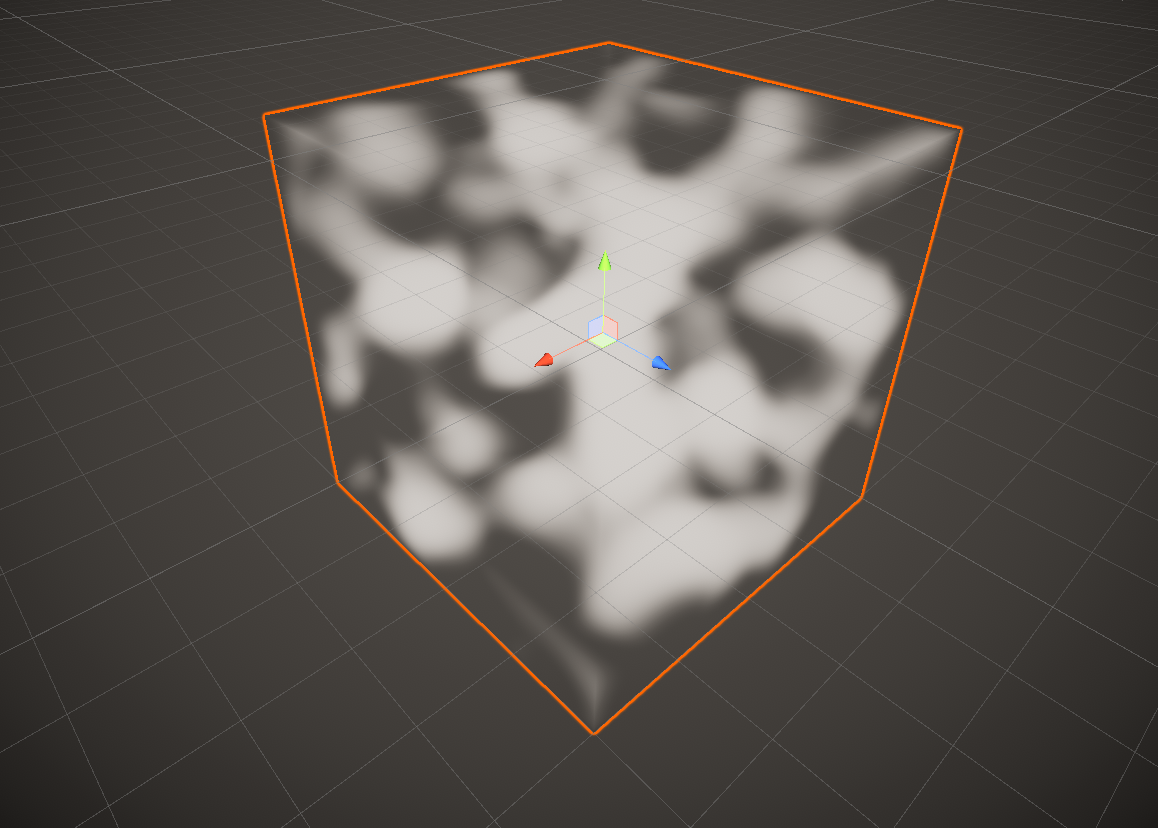
\includegraphics[width=\linewidth]{unity captures/prototype1.PNG}
    \captionof{figure}{Prototype: Rendered image of sampled density based on 3D Perlin noise.}
    \label{img:captures:prototype1}
\end{figure}

\noindent
With this first try, a Perlin noise function was sampled. The returned value had to be normalized in a range of $[0, 1]$ in order to for it to be used as alpha value of the color.

\subsubsection{Normalizing Density}
This is where the exponential function $exp(x) = e^{-x}$ comes in, which (when clamped from 0 to 1) converts very low values to 1.0 and higher values will converge towards 0.0.

\begin{figure}[H]
    \centering
    \begin{minipage}{0.47\linewidth}
        \begin{tikzpicture}
            \begin{axis}[
                axis lines=center,
                samples=50,
                xmin=-0.5,
                xmax=4.5,
                ymin=-0.2,
                ymax=1.2,
                xlabel={$x$},
                ylabel={$y$},
                xlabel style={below right},
                ylabel style={above left},
                height=4cm,
                width=8cm,
                ytick={0,1},
                xtick={0,1,2,3,4},
                ]
    
                \addplot[red] plot (\x, { exp(-\x)) });
            \end{axis}
        \end{tikzpicture}
        \captionof{figure}{Exponential function $exp(x) = e^{-x}$.}
        \label{img:math:exp}
    \end{minipage}        
    \hfill
    \begin{minipage}{0.47\linewidth}
        \begin{tikzpicture}
            \begin{axis}[
                axis lines=center,
                samples=50,
                xmin=-0.5,
                xmax=4.5,
                ymin=-0.2,
                ymax=1.2,
                xlabel={$x$},
                ylabel={$y$},
                xlabel style={below right},
                ylabel style={above left},
                height=4cm,
                width=8cm,
                ytick={0,1},
                xtick={0,1,2,3,4},
                ]
    
                \addplot[red] plot (\x, { 1 - exp(-\x)) });
            \end{axis}
        \end{tikzpicture}
        \captionof{figure}{Inverted exponential function $exp'(x) = 1 - e^{-x}$.}
        \label{img:math:exp1}       
    \end{minipage}
\end{figure}

\noindent
When inverting $exp(x)$, the function $exp'(x)$ returns a value that can be directly used for the transparency of the cloud. The denser it gets, the more opaque it will be.

\clearpage
\subsection{Improving Noise}
After further experimenting with the noise sampling function, the idea arose to combine Perlin and Voronoi noise, which hopefully would create a more distinguished, random pattern.
The final sampling function simply multiplies both noise values at a given point \lstinline[language=HLSL]{position}. 

\begin{lstlisting}[language=HLSL, numbers=left, caption=Implementation of a density sampling function., label=lst:shader:prototype:sampledensity]
float sampleDensity(float3 position) {
  float3 vpos = position * _VoronoiScale + _VoronoiOffset;
  float3 ppos = position * _PerlinScale + _PerlinOffset;
  float vd = getColorVoronoi(vpos, _VoronoiOctaves, _VoronoiPersistance));
  float pd = getColorPerlin(ppos, _PerlinOctaves, _PerlinPersistance));
  
  vd = max(0, vd - _VoronoiDensityThreshold) * _VoronoiDensityMultiplier;
  pd = max(0, pd - _PerlinDensityThreshold) * _PerlinDensityMultiplier;
  
  // fix boost density by factor 2
  float density = vd * pd * 2.0;
  return density;
}
\end{lstlisting}

\noindent
By adjusting some of the \gls{parameters} and increasing the octaves of both noises, a more patchy and cloudy look can be achieved at the cost of performance.

\begin{figure}[H]
    \centering
    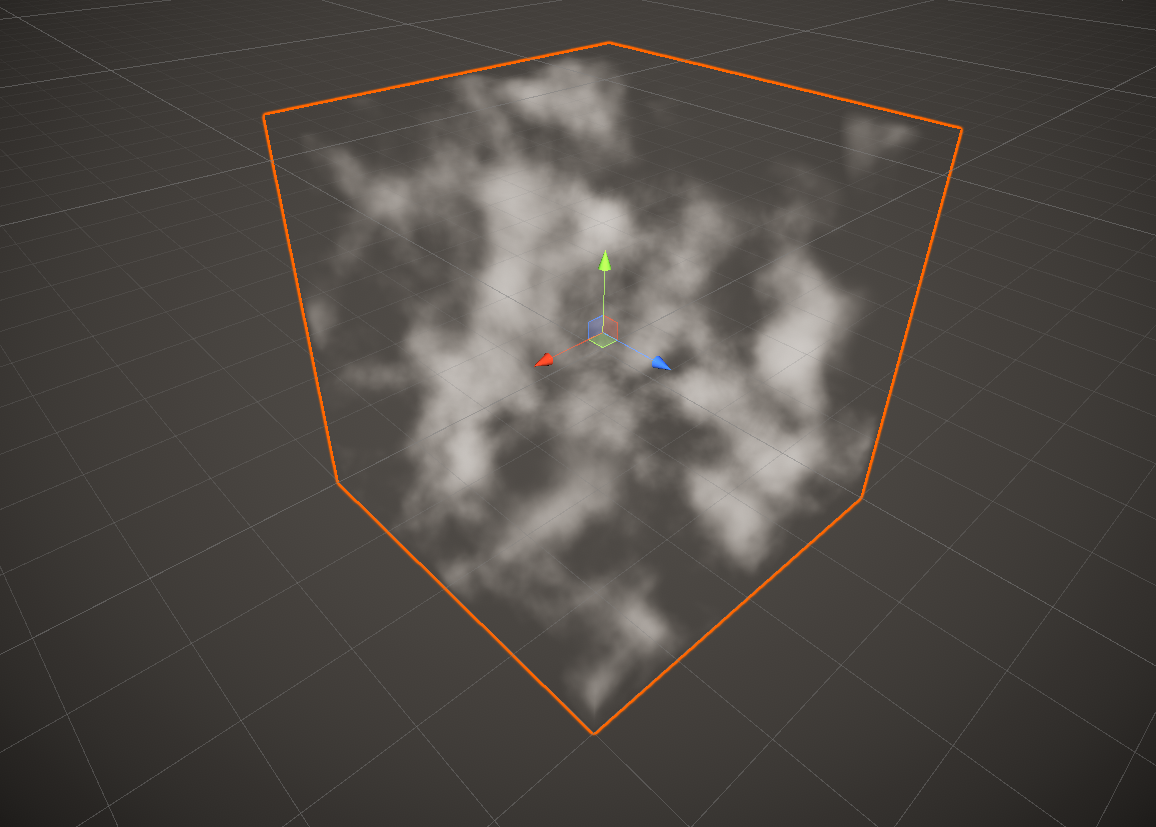
\includegraphics[width=\linewidth]{unity captures/prototype2.PNG}
    \captionof{figure}{Prototype: Rendered image of sampled density based on mixed noises.}
    \label{img:captures:prototype2}
\end{figure}

\clearpage
\subsection{Light Transmittance and Light Scattering}
One of the more prominent lighting features of clouds is its translucency. It describes how light bounces and scatters inside the matter, then exits at a different point. This is called \textit{\gls{sss}} (SSS).
It results in illuminated areas where the cloud is thin. In nature, \gls{sss} is a very complex and computationally demanding process. For computer graphics however, it is often either simplified or substituted with some other algorithm that produces a similar outcome at lower performance cost.

\subsubsection{Sunlight Forwarding}
When approaching the implementation of \gls{sss} and directional lighting, it seemed most reasonable to start with the sun being visible behind the clouds, or at least shining through them.
This implies finding a way to illuminate clouds that cover the sun.
\\
After some consideration and brainstorming, the following method was chosen to solve the issue:

\begin{figure}[H]
    \centering
    \begin{tikzpicture}[scale=1.2]
        \tikzset{edge/.style = {-{Latex[length=3mm]},shorten >= -4pt}}
        \tikzset{shortedge/.style = {-{Latex[length=3mm]},shorten <=-4pt,shorten >= -4pt}}
        \tikzset{line/.style = {shorten >=-4pt}}
        \tikzset{icon/.style = {font=\Large}}

        % icons
        \node[icon,rotate=35,anchor=west] (cam) at (0, 0) {\faVideoCamera};
        \node[icon] (light) at (8, 6) {\faLightbulbO};
        \node at (8, 6.5) {light source};

        % clouds
        \node (cloud) at (4.5, 5.2) {};
        \node[cloud, cloud puffs=15.7, cloud, minimum width=3.5cm, minimum height=2.2cm, align=center, draw] (cloud) at (cloud) {};

        % screen space
        \draw (1,1) -- (5,1) -- (5,4);

        % rays
        \node[red] (p1) at (3, 2.25) {\ding{53}};
        \node (p2) at (5, 3.75) {};
        
        \node[cyan,,mark=x] (c1) at (2.31, 2.4) {\ding{53}};
        \node (c2) at (3.7, 4) {};
        \node[cyan] (c3) at (4.7, 5.35) {\textbullet};

        \draw[red, line] (cam) -- (p1);
        \draw[red, line, loosely dashed] (p1) -- (p2);
        \draw[red, edge, loosely dashed] (p2) -- (light);
        
        \draw[cyan, line] (cam) -- (c1);
        \draw[cyan, line, loosely dashed] (c1) -- (c2);
        \draw[cyan, edge, loosely dashed] (c2) -- (c3);

        % rest of screen space
        \draw (5,4) -- (1,4) node[anchor=south west] {screen space} -- (1,1);

        \end{tikzpicture}
    \captionof{figure}{Sunlight transmittance sampling (1).}
    \label{img:tikz:prototypes:sunlight}
\end{figure}

\noindent
asdasdasdasd
asdasdasdasddas
draftsdas
distancedsa


\begin{figure}[H]
    \centering
    \begin{tikzpicture}[scale=1.2]
        \tikzset{edge/.style = {-{Latex[length=3mm]},shorten >= -4pt}}
        \tikzset{shortedge/.style = {-{Latex[length=3mm]},shorten <=-4pt,shorten >= -4pt}}
        \tikzset{lightedge1/.style = {-{Latex[length=3mm]},shorten <=-4pt,shorten >= 1cm}}
        \tikzset{lightedge2/.style = {-{Latex[length=3mm]},shorten <=-4pt,shorten >= 1cm}}
        \tikzset{lightedge3/.style = {-{Latex[length=3mm]},shorten <=-4pt,shorten >= 1cm}}
        \tikzset{icon/.style = {font=\Large}}

        % icons
        \node[icon,rotate=35,anchor=west] (cam) at (0, 0) {\faVideoCamera};
        \node[icon] (light) at (1, 6) {\faLightbulbO};
        \node at (1, 6.5) {light source};

        % clouds
        \node (cloud) at (4.5, 3.5) {};
        \node[cloud, cloud puffs=15.7, cloud ignores aspect, minimum width=5cm, minimum height=3.5cm, align=center, draw] (cloud) at (cloud) {};

        % outer point
        \node (pOut) at (7, 5.25) {};

        % rays
        \draw[red, edge] (cam) -- (pOut) node[midway,above,sloped,xshift=-3cm] {};
        
        % cloud points
        \node[red] (p1) at (3.5, 2.625) {\textbullet};
        \node[red] (p2) at (4.5, 3.375) {\textbullet};
        \node[red] (p3) at (5.5, 4.125) {\textbullet};
        \node[red] (p4) at (4.5, 3.375) {\textbullet};
        \node[red] (p5) at (5.5, 4.125) {\textbullet};

        % light march rays
        \draw[cyan, lightedge1] (p1) -- (light) node[midway,above,sloped] {};
        \draw[cyan, lightedge2] (p2) -- (light) node[midway,above,sloped] {};
        \draw[cyan, lightedge3] (p3) -- (light) node[midway,above,sloped] {$R_{light}$};

        % light sample points
        \node[cyan] (l1) at (3.25, 2.95) {\textbullet};
        \node[cyan] (l2) at (4.15, 3.625) {\textbullet};
        \node[cyan] (l3) at (5.0, 4.325) {\textbullet};
        
        \node[cyan] (l5) at (3.0, 3.3) {\textbullet};
        \node[cyan] (l6) at (3.75, 3.95) {\textbullet};
        \node[cyan] (l7) at (4.5, 4.55) {\textbullet};
        
        \node[cyan] (l8) at (2.75, 3.65) {\textbullet};
        \node[cyan] (l9) at (3.35, 4.22) {\textbullet};
        \node[cyan] (l10) at (3.95, 4.775) {\textbullet};

        \end{tikzpicture}
    \captionof{figure}{Sunlight transmittance sampling (1).}
    \label{img:tikz:prototypes:lightmarching1}
\end{figure}

\begin{figure}[H]
    \centering
    \begin{tikzpicture}[scale=1.2]
        \tikzset{edge/.style = {-{Latex[length=3mm]},shorten >= -4pt}}
        \tikzset{shortedge/.style = {-{Latex[length=3mm]},shorten <=-4pt,shorten >= -4pt}}
        \tikzset{lightedge1/.style = {-{Latex[length=3mm]},shorten <=-4pt,shorten >= 1cm}}
        \tikzset{lightedge2/.style = {-{Latex[length=3mm]},shorten <=-4pt,shorten >= 1cm}}
        \tikzset{lightedge3/.style = {-{Latex[length=3mm]},shorten <=-4pt,shorten >= 1cm}}
        \tikzset{icon/.style = {font=\Large}}

        % icons
        \node[icon,rotate=35,anchor=west] (cam) at (0, 0) {\faVideoCamera};
        \node[icon] (light) at (1, 6) {\faLightbulbO};
        \node at (1, 6.5) {light source};

        % clouds
        \node (cloud) at (4.5, 3.5) {};
        \node[cloud, cloud puffs=15.7, cloud ignores aspect, minimum width=5cm, minimum height=3.5cm, align=center, draw] (cloud) at (cloud) {};

        % outer point
        \node (pOut) at (7, 5.25) {};

        % rays
        \draw[red, edge] (cam) -- (pOut) node[midway,above,sloped,xshift=-3cm] {};
        
        % cloud points
        \node[red] (p1) at (3.5, 2.625) {\textbullet};
        \node[red] (p2) at (4.5, 3.375) {\textbullet};
        \node[red] (p3) at (5.5, 4.125) {\textbullet};
        \node[red] (p4) at (4.5, 3.375) {\textbullet};
        \node[red] (p5) at (5.5, 4.125) {\textbullet};

        % light march rays
        \draw[cyan, lightedge1] (p1) -- (light) node[midway,above,sloped] {};
        \draw[cyan, lightedge2] (p2) -- (light) node[midway,above,sloped] {};
        \draw[cyan, lightedge3] (p3) -- (light) node[midway,above,sloped] {$R_{light}$};

        % light sample points
        \node[cyan] (l1) at (3.25, 2.95) {\textbullet};
        \node[cyan] (l2) at (4.15, 3.625) {\textbullet};
        \node[cyan] (l3) at (5.0, 4.325) {\textbullet};
        
        \node[cyan] (l5) at (3.0, 3.3) {\textbullet};
        \node[cyan] (l6) at (3.75, 3.95) {\textbullet};
        \node[cyan] (l7) at (4.5, 4.55) {\textbullet};
        
        \node[cyan] (l8) at (2.75, 3.65) {\textbullet};
        \node[cyan] (l9) at (3.35, 4.22) {\textbullet};
        \node[cyan] (l10) at (3.95, 4.775) {\textbullet};

        \end{tikzpicture}
    \captionof{figure}{Sunlight transmittance sampling  (2).}
    \label{img:tikz:prototypes:lightmarching2}
\end{figure}